%%%%%%%%%%%%%%%%%%%%%%%%%%%%%%%%%%%%%%%%%%%%%%%%%%%%%%%%%%%%%%%%%%%%%%%%%%%%%%%%
%2345678901234567890123456789012345678901234567890123456789012345678901234567890
%        1         2         3         4         5         6         7         8
\documentclass[letterpaper, 10 pt, conference]{ieeeconf}  % Comment this line out if you need a4paper
\usepackage{times}
\usepackage{graphicx}
\usepackage{subcaption}
\usepackage{amsmath}
\usepackage{amssymb}
\usepackage{amsfonts}
\usepackage{comment}
\usepackage{color}
% numbers option provides compact numerical references in the text. 
\usepackage{multicol}
\usepackage{booktabs}
\usepackage[bookmarks=true]{hyperref}
\usepackage[font=small,labelfont=bf]{caption}
\newtheorem{theorem}{Theorem}
\newtheorem{corollary}{Corollary}[theorem]
\newtheorem{lemma}[theorem]{Lemma}
%\documentclass[a4paper, 10pt, conference]{ieeeconf}      % Use this line for a4 paper
\IEEEoverridecommandlockouts                              % This command is only needed if 
                                                          % you want to use the \thanks command
\overrideIEEEmargins                                      % Needed to meet printer requirements.

\title{\LARGE \bf 
	Paper Title}

\begin{document}
\maketitle
\thispagestyle{empty}
\pagestyle{empty}
%%%%%%%%%%%%%%%%%%%%%%%%%%%%%%%%%%%%%%%
\begin{abstract}
Abstract
%1. The problem background
%2. The Major Challenge
%3. Our Solution
%4. Major Contribution
\end{abstract}
\section{INTRODUCTION}
\label{sec:introduction}
\begin{figure}
	\centering
	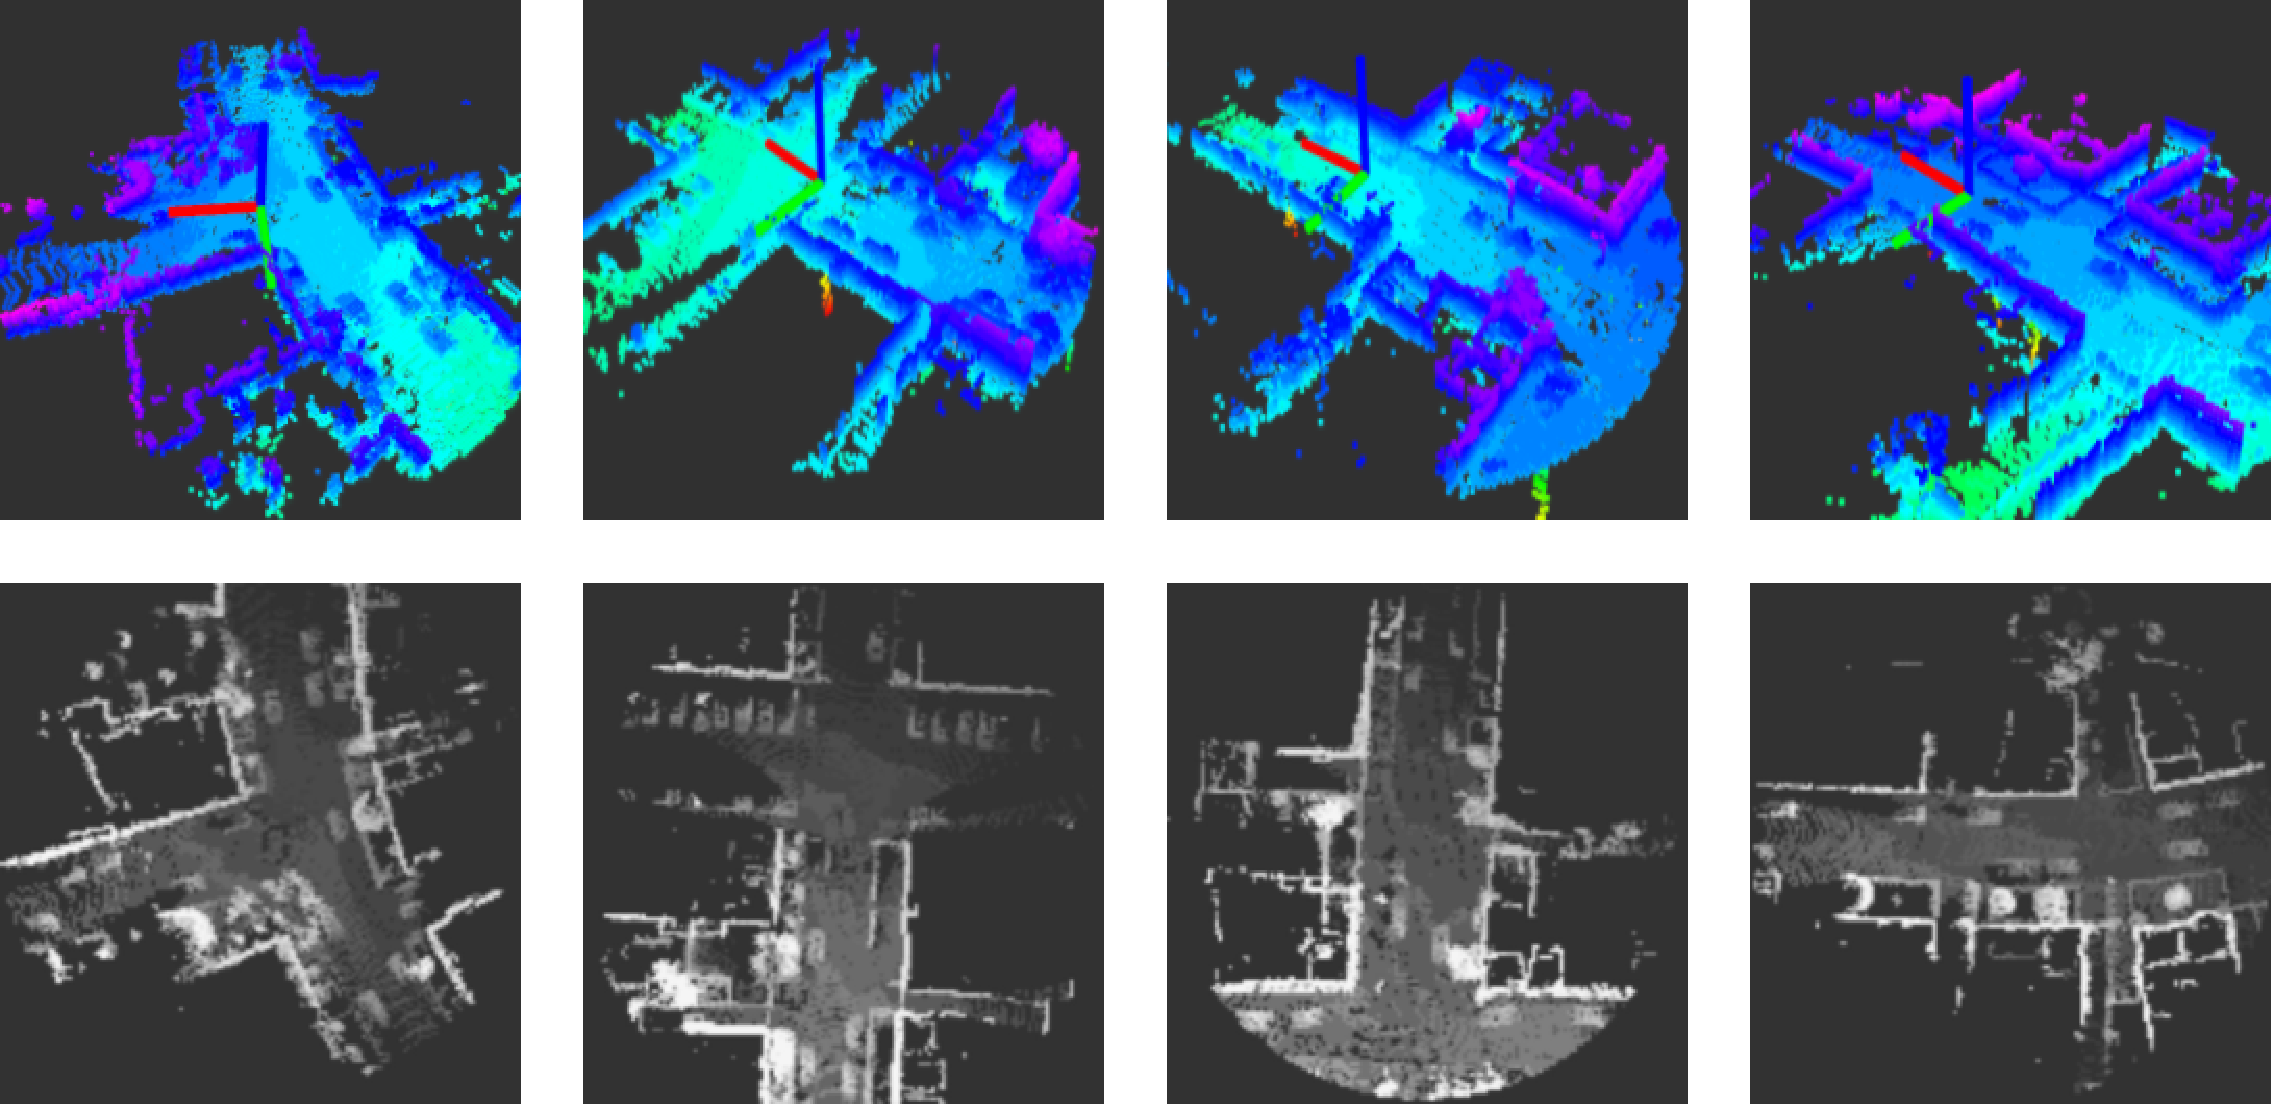
\includegraphics[width=0.9\linewidth]{figures/obm.pdf}
	\caption{The figure.}
	\label{fig:obm}
\end{figure}


\section{Multi-Resolution Particle Filter}
\label{sec:method}
\section{Experiments}
\label{sec:experiments}
\section{CONCLUSIONS}
\label{sec:conclusion}
\addtolength{\textheight}{-12cm}  
\begin{thebibliography}{99}
\bibitem{1} B. Grocholsky and J. Keller, “Cooperative Air and Ground Survaillance Cooperative Air and Ground Survaillance,” vol. 13, no. 2006, pp. 16–25, 2007.
\end{thebibliography}

%%%%%%%%%%%%%%%%%%%%%%%%%%%%%%%%%%%%%%%%%%%%%%%%%%%%%%%%%%%%%%%%%%%%%%%%%%%%%%%%
\end{document}
